\documentclass[tikz,border=12pt]{standalone}
% Shared visual language for standalone EMT block diagrams.
\usepackage{amsmath}
\usetikzlibrary{arrows.meta,backgrounds,calc,fit,positioning}

\tikzset{
    emt diagram/.style = {>={Stealth[length=2.4mm]}},
    line/.style        = {semithick, rounded corners=6pt},
    block/.style       = {draw, semithick, fill=white,
                          minimum height=1cm, minimum width=2.3cm},
    hblock/.style      = {block, minimum width=2.24cm, minimum height=1.3cm},
    vblock/.style      = {block, minimum width=1.3cm, minimum height=2.24cm},
    sum/.style         = {draw, semithick, fill=white, circle,
                          inner sep=2.6pt},
    signal/.style      = {circle, fill, inner sep=1.4pt,
                          label distance=3pt},
    sig/.style         = {font=\small},
    pm/.style          = {font=\scriptsize},
    wire jump/.style   = {line,
                          preaction={draw=white, line width=3pt,
                                     line cap=round}},
    enclosure/.style   = {draw, dashed, semithick, rounded corners=4pt},
    operator enclosure/.style = {enclosure, inner xsep=7mm, inner ysep=6mm}
}


\begin{document}
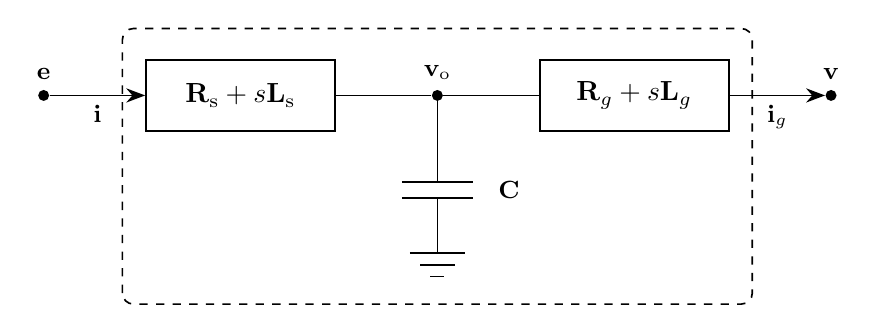
\begin{tikzpicture}[emt diagram]

% ================= Series branches =================
\node[block, minimum width=2.4cm, minimum height=0.9cm]
    (source) at (-2.5, 0) {$\mathbf{R}_{\mathrm{s}} + s\mathbf{L}_{\mathrm{s}}$};
\node[block, minimum width=2.4cm, minimum height=0.9cm]
    (grid) at (2.5, 0) {$\mathbf{R}_g + s\mathbf{L}_g$};
\node[signal, label={[sig]above:$\mathbf{e}$}] (e) at (-5.0, 0) {};
\node[signal, label={[sig]above:$\mathbf{v}$}] (v) at (5.0, 0) {};
\node[signal, label={[sig]above:$\mathbf{v}_{\mathrm{o}}$}] (vo) at (0, 0) {};
\draw[->, line] (e) -- node[sig, below] {$\mathbf{i}$} (source.west);
\draw[line] (source.east) -- (vo) -- (grid.west);
\draw[->, line] (grid.east) -- node[sig, below] {$\mathbf{i}_g$} (v);

% ================= Shunt capacitor =================
\draw[line] (vo) -- (0, -1.1);
\draw[semithick] (-0.45, -1.1) -- (0.45, -1.1);
\draw[semithick] (-0.45, -1.3) -- (0.45, -1.3);
\node[sig, anchor=west] at (0.65, -1.2) {$\mathbf{C}$};
\draw[line] (0, -1.3) -- (0, -2.0);
\draw[semithick] (-0.35, -2.0) -- (0.35, -2.0);
\draw[semithick] (-0.22, -2.15) -- (0.22, -2.15);
\draw[semithick] (-0.09, -2.3) -- (0.09, -2.3);

% ================= Model enclosure =================
\draw[enclosure] (-4.0, -2.65) rectangle (4.0, 0.85);

\end{tikzpicture}
\end{document}
